\chapter{HIỆN THỰC CÁC NGHIỆP VỤ NÂNG CAO}

Chương này đi sâu vào các giải pháp kỹ thuật phức tạp đã được thiết kế và hiện thực hóa trong hệ thống BrewLite nhằm giải quyết các bài toán hóc búa về tính toàn vẹn dữ liệu, kiểm soát đồng thời và độ tin cậy giao dịch trong môi trường đa người dùng.

\section{Máy trạng thái Đơn hàng (Order State Machine)}
Quy trình luân chuyển trạng thái của một đơn hàng trong BrewLite được quản lý chặt chẽ thông qua mô hình Máy trạng thái hữu hạn (\textit{Finite State Machine}), định nghĩa nguyên văn trong tập tin mã nguồn \texttt{backend/src/modules/orders/order-state.ts}.

Sơ đồ máy trạng thái đơn hàng được trình bày chi tiết tại Hình~\ref{fig:order-state-machine}.

\begin{figure}[htbp]
    \centering
    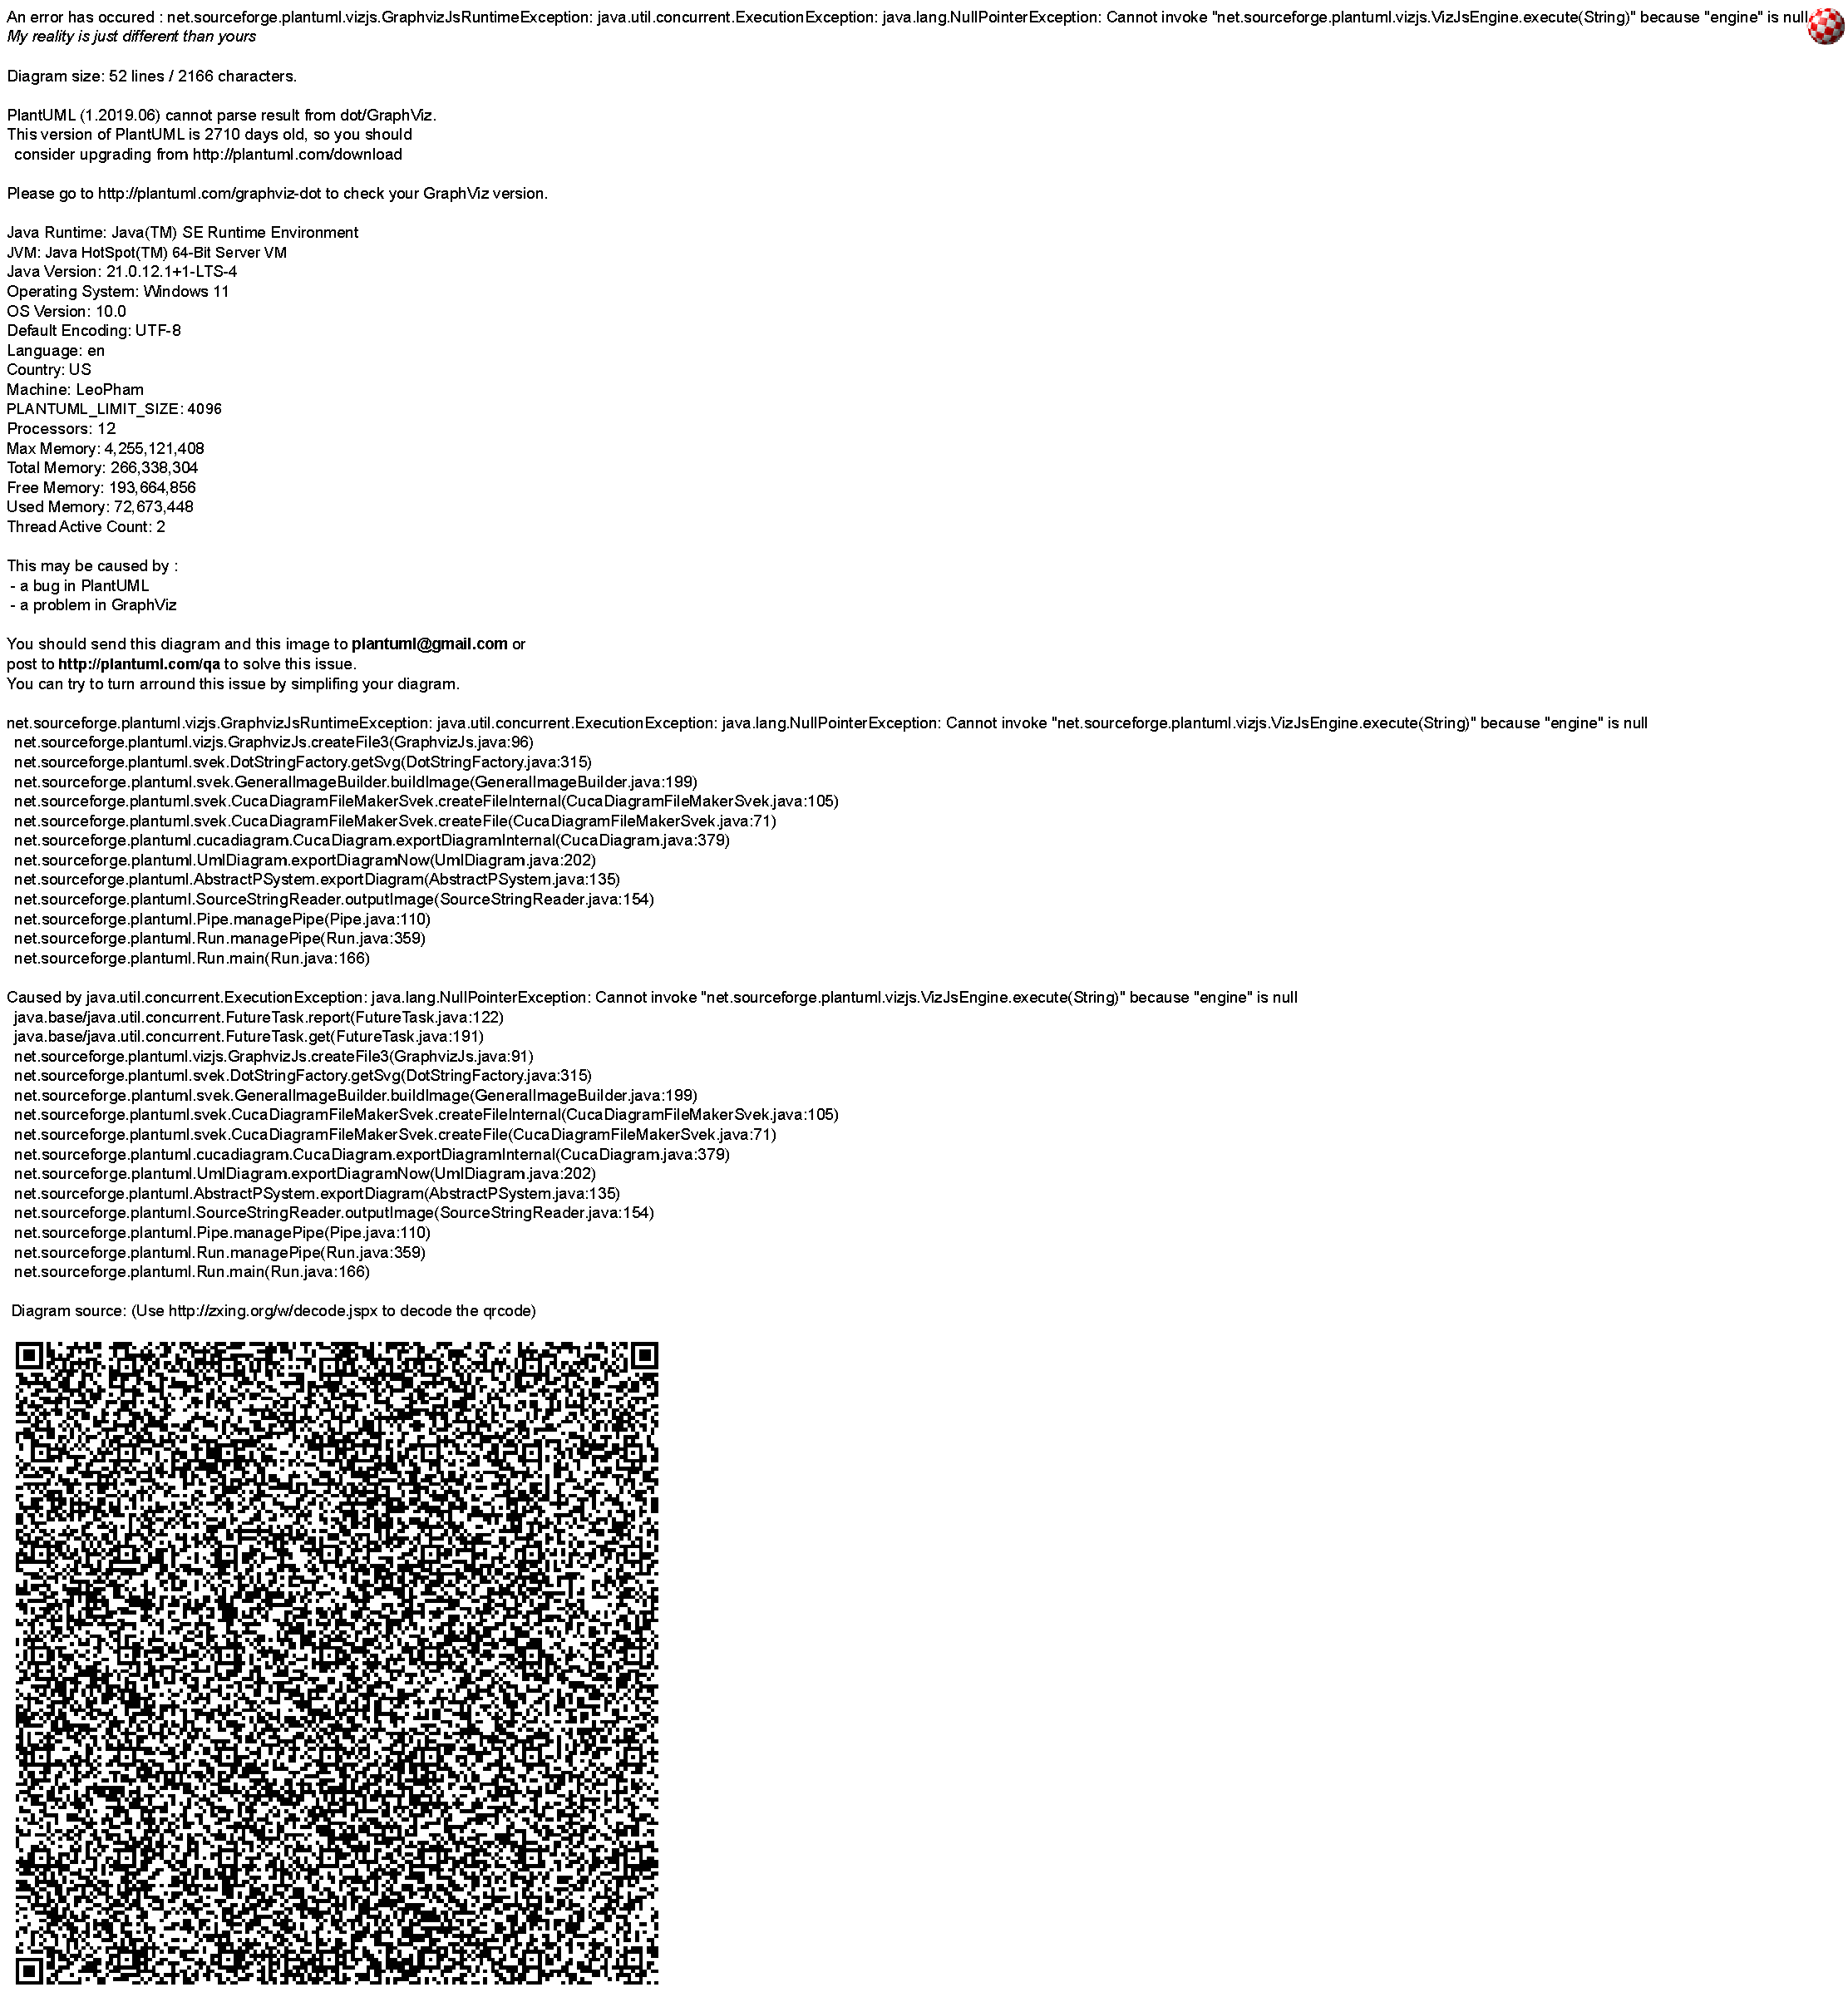
\includegraphics[width=0.88\textwidth]{figures/order-state-machine.pdf}
    \caption{Sơ đồ Máy trạng thái Đơn hàng BrewLite (9 chuyển tiếp hợp lệ)}
    \label{fig:order-state-machine}
\end{figure}

Hệ thống quy định chính xác \textbf{9 chuyển tiếp trạng thái hợp lệ} giữa 7 trạng thái nghiệp vụ:
\begin{enumerate}
    \item \texttt{PENDING \(\to\) PAID}: Chuyển đổi khi khách hàng thực hiện thanh toán trực tuyến thành công qua cổng thanh toán.
    \item \texttt{PENDING \(\to\) PAYMENT\_FAILED}: Chuyển đổi khi giao dịch thanh toán bị từ chối, thẻ hết hạn hoặc phát sinh lỗi mạng.
    \item \texttt{PENDING \(\to\) CANCELLED}: Khách hàng chủ động hủy đơn khi chưa thanh toán hoặc đơn hàng hết thời gian chờ (timeout).
    \item \texttt{PAID \(\to\) PREPARING}: Quầy pha chế (Barista) tiếp nhận đơn hàng đã thanh toán và bắt đầu quy trình làm đồ uống.
    \item \texttt{PAID \(\to\) CANCELLED}: Đơn hàng đã thanh toán bị hủy do sự cố bất khả kháng (ví dụ hết nguyên liệu đột xuất), kích hoạt luồng hoàn tiền.
    \item \texttt{PREPARING \(\to\) READY}: Nhân viên pha chế hoàn tất đồ uống, đơn hàng sẵn sàng chờ khách hàng đến nhận tại quầy.
    \item \texttt{READY \(\to\) COMPLETED}: Khách hàng nhận đồ uống thành công. Đây là một trong hai trạng thái kết thúc (\textit{Terminal State}).
    \item \texttt{PAYMENT\_FAILED \(\to\) PENDING}: Khách hàng nhấn thử lại (\textit{Retry Payment}), chọn phương thức thanh toán mới để tiến hành trả tiền lại cho đơn hàng.
    \item \texttt{PAYMENT\_FAILED \(\to\) CANCELLED}: Đơn hàng bị hủy vĩnh viễn sau khi thanh toán thất bại và khách hàng không có nhu cầu thử lại.
\end{enumerate}

Hai trạng thái \texttt{COMPLETED} và \texttt{CANCELLED} là trạng thái kết thúc vĩnh viễn (\textit{Terminal States}), danh sách chuyển tiếp tiếp theo là mảng rỗng (\texttt{[]}). Bất kỳ nỗ lực chuyển đổi sai quy tắc nào đều bị chặn ngay lập tức bởi hàm kiểm tra \texttt{assertTransition()} và ném ngoại lệ \texttt{409 ConflictException}:
\begin{lstlisting}[language=Java]
export function assertTransition(fromStatus: OrderStatus, toStatus: OrderStatus): void {
  const allowedStatuses = ALLOWED_TRANSITIONS[fromStatus];
  if (!allowedStatuses?.includes(toStatus)) {
    throw new ConflictException(
      `Invalid order status transition: ${fromStatus} -> ${toStatus}`
    );
  }
}
\end{lstlisting}

\section{Xử lý Thanh toán Bất biến (Idempotent Payment)}
Trong môi trường mạng không ổn định, khách hàng thường có xu hướng nhấp đúp vào nút "Thanh toán" hoặc trình duyệt tự động gửi lại request khi mạng chập chờn (\textit{Network Timeout}). Nếu không có cơ chế bảo vệ, người dùng sẽ bị trừ tiền nhiều lần cho cùng một đơn hàng (\textit{Double Charge}).

BrewLite giải quyết triệt để vấn đề này bằng cơ chế \textbf{Idempotency} cấp độ doanh nghiệp:
\begin{enumerate}
    \item \textbf{Sinh khóa định danh duy nhất (\texttt{Idempotency-Key}):} Mỗi khi người dùng bấm xác nhận thanh toán, client tự động sinh một mã UUIDv4 duy nhất và đính kèm vào HTTP Header: \texttt{Idempotency-Key: <UUID>}.
    \item \textbf{Mã hóa toàn vẹn dữ liệu (\texttt{request\_hash}):} Backend nhận request và tính toán mã băm SHA-256 trên nội dung JSON của request body. Mã băm này đại diện cho tính nguyên vẹn của giao dịch.
    \item \textbf{Kiểm tra và Điều phối giao dịch:}
    \begin{itemize}
        \item \textbf{Trường hợp 1 (Trùng lặp thành công - Replay):} Nếu \texttt{idempotency\_key} đã tồn tại trong bảng \texttt{payments} và có trạng thái \texttt{SUCCESS}, hệ thống lập tức trả về kết quả đã lưu trước đó mà không thực hiện gọi sang Mock Gateway.
        \item \textbf{Trường hợp 2 (Xung đột đồng thời - Concurrent Request):} Nếu \texttt{idempotency\_key} đang ở trạng thái \texttt{PENDING} (giao dịch trước đó đang xử lý dở dang), hệ thống lập tức từ chối và ném lỗi \texttt{409 Conflict}.
        \item \textbf{Trường hợp 3 (Sai lệch tải trọng - Payload Tampering):} Nếu \texttt{idempotency\_key} trùng nhưng \texttt{request\_hash} khác nhau (ví dụ cố tình gửi cùng key nhưng đổi số tiền hoặc ID đơn hàng), hệ thống ném lỗi \texttt{422 Unprocessable Entity}.
        \item \textbf{Trường hợp 4 (Giao dịch mới):} Bản ghi thanh toán được tạo với trạng thái \texttt{PENDING}, gọi cổng thanh toán, sau đó cập nhật kết quả cuối cùng.
    \end{itemize}
\end{enumerate}

\section{Kiểm soát Đồng thời Tồn kho (Concurrency Control)}
Một trong những thách thức lớn nhất của các ứng dụng thương mại điện tử là bài toán xung đột tồn kho (\textit{Race Condition}) khi nhiều khách hàng cùng đặt mua sản phẩm cuối cùng vào cùng một thời điểm.

BrewLite áp dụng kỹ thuật \textbf{Khóa lạc quan (Optimistic Locking)} kết hợp cùng \textbf{Interactive Transaction (\texttt{prisma.\$transaction})}:
\begin{itemize}
    \item Trên bảng \texttt{products}, mỗi dòng sản phẩm có một trường số nguyên \texttt{version} với giá trị khởi tạo là \texttt{0}.
    \item Khi giao dịch tạo đơn hàng diễn ra, câu lệnh cập nhật số lượng tồn kho bắt buộc phải thỏa mãn điều kiện phiên bản không bị thay đổi:
    \begin{lstlisting}[language=SQL]
UPDATE products
SET stock = stock - :quantity,
    version = version + 1
WHERE id = :productId 
  AND version = :currentVersion 
  AND stock >= :quantity;
    \end{lstlisting}
    \item Nếu hai giao dịch đồng thời cùng đọc phiên bản \(version = 0\), giao dịch thứ nhất thực thi thành công sẽ đẩy phiên bản lên \(version = 1\). Giao dịch thứ hai khi cập nhật sẽ nhận số dòng bị ảnh hưởng là 0 (\texttt{affected\_rows = 0}).
    \item Khi phát hiện số dòng cập nhật bằng 0, hệ thống ngay lập tức ném lỗi \texttt{409 ConflictException} ("Sản phẩm vừa có thay đổi, vui lòng thử lại"), đồng thời tự động rollback toàn bộ giao dịch tạo đơn, đảm bảo tồn kho tuyệt đối không bao giờ bị âm.
\end{itemize}

\section{Nghiệp vụ Khuyến mãi và Điểm tích lũy Thành viên}
Hệ thống tích hợp bộ đôi động cơ khuyến mãi và khách hàng thân thiết hoạt động nhịp nhàng nhằm gia tăng giá trị đơn hàng:

\subsection{Cơ chế Mã giảm giá (Promotions Engine)}
Hệ thống hỗ trợ cấu hình mã giảm giá đa dạng được quản lý trong bảng \texttt{promotions}. Tiêu biểu là mã ưu đãi \texttt{WELCOME10}:
\begin{itemize}
    \item \textbf{Mã code:} \texttt{WELCOME10}.
    \item \textbf{Tỷ lệ chiết khấu:} Giảm 10\% trên tổng giá trị tạm tính của đơn hàng (\texttt{total\_amount}).
    \item \textbf{Điều kiện áp dụng:} Giá trị đơn hàng tối thiểu (\texttt{min\_order\_amount}) phải đạt từ 100.000 VNĐ trở lên.
    \item \textbf{Mức giảm tối đa:} Giới hạn mức chiết khấu tối đa (\texttt{max\_discount}) là 50.000 VNĐ.
    \item Công thức tính:
    \[
    \text{discountAmount} = \min\left( \text{totalAmount} \times 10\%, 50.000 \right)
    \]
\end{itemize}

\subsection{Cơ chế Điểm thưởng Thành viên (Loyalty Points)}
\begin{itemize}
    \item \textbf{Tích lũy điểm (Earn Points):} Với mỗi đơn hàng được thanh toán thành công, khách hàng được tích lũy 1 điểm thưởng cho mỗi 10.000 VNĐ giá trị thực trả (\texttt{finalAmount}):
    \[
    \text{pointsEarned} = \left\lfloor \frac{\text{finalAmount}}{10.000} \right\rfloor
    \]
    \item \textbf{Quy đổi điểm (Redeem Points):} Khách hàng có thể sử dụng điểm tích lũy để trừ trực tiếp vào đơn hàng mới. Giá trị quy đổi là \(1 \text{ điểm} = 1.000 \text{ VNĐ}\). Nhằm đảm bảo an toàn doanh thu, hệ thống đặt ra quy tắc cứng: số tiền giảm từ điểm thưởng tối đa không được vượt quá 50\% giá trị đơn hàng sau khi đã trừ mã giảm giá.
    \item Mọi biến động cộng/trừ điểm đều được ghi vết minh bạch trong bảng \texttt{loyalty\_transactions}.
\end{itemize}
